\chapter{Economic Aspect of Operating Systems (Florian Prandstetter)}
\label{chap:Economic_aspect_of_Operating_Systems}

\section{Introduction}

In this section, the relevance of Operating Systems in our economy will be discussed. The importance of OS in our daily life is not always obvious.
The OS is the most important software on a computer. It manages the computer's memory, processes, and all of its software and hardware. 
With the rising amount of digitalization, the OS is also becoming more important than ever.

To get an overview of what an OS is, please refer to Chapter \ref{sec:WhatIsAnOs}.

\section{Operating System Market Share}

The OS market is dominated by four major players: Android, Microsoft Windows, Linux, and macOS.
The market share of the Operating Systems is shown in Figure \ref{fig:Operating_Systems_Market_Share}. 

In recent years, the market share of Android has been increasing. This is due to the rising number of smartphones and tablets.
Microsoft Windows is still the most used OS on desktops and laptops.

\begin{figure}[H]
    \centering
    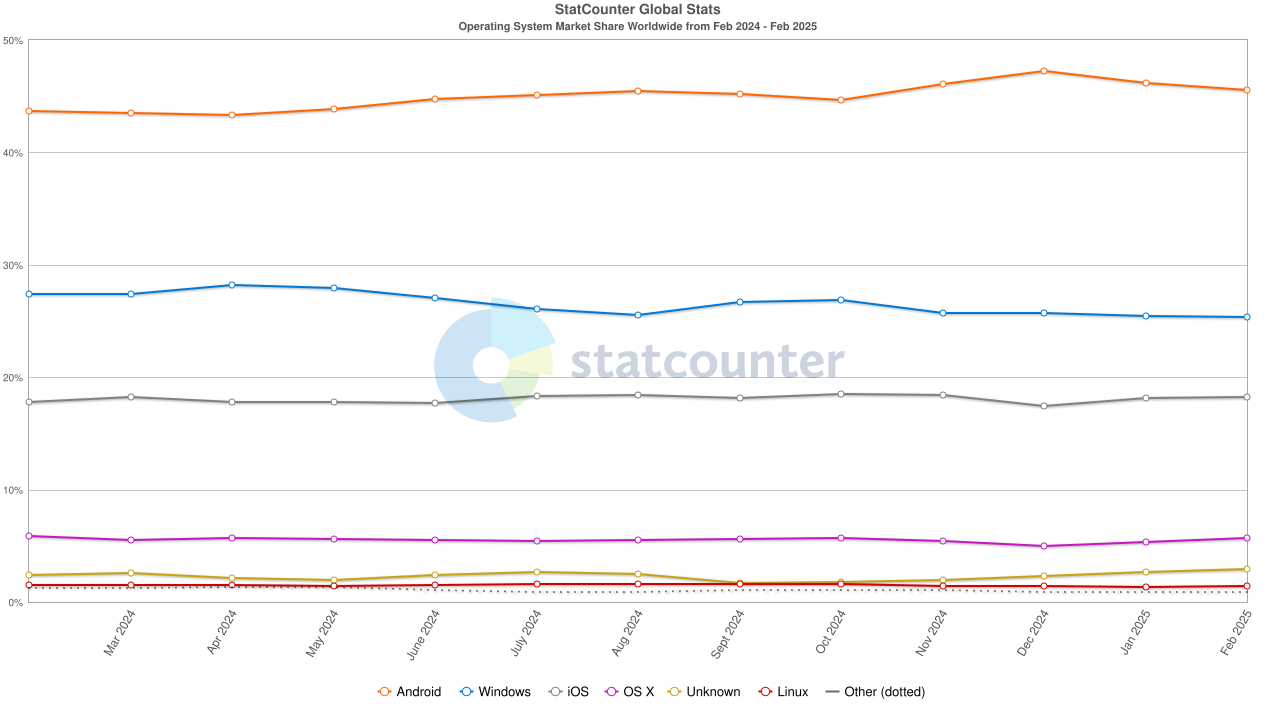
\includegraphics[width=0.8\textwidth]{figures/StatCounter-os_combined-ww-monthly-202402-202502.png}
    \caption{Operating Systems Market Share}
    \label{fig:Operating_Systems_Market_Share}
\end{figure}
\cite{OsMarketShare2}

The global market of Operating Systems is expected to reach \textdollar 48.18 billion at a CAGR of 1.9\% in 2026. 
\cite{OsMarketShare3}

\cite{OsMarketShare}
\cite{OsWikipedia}

\subsection{Operating Systems for Servers}

When looking at the Operating Systems used for web servers, the market share looks very different.
The two main competitors are Microsoft and Red Hat. 

\begin{figure}[H]
    \centering
    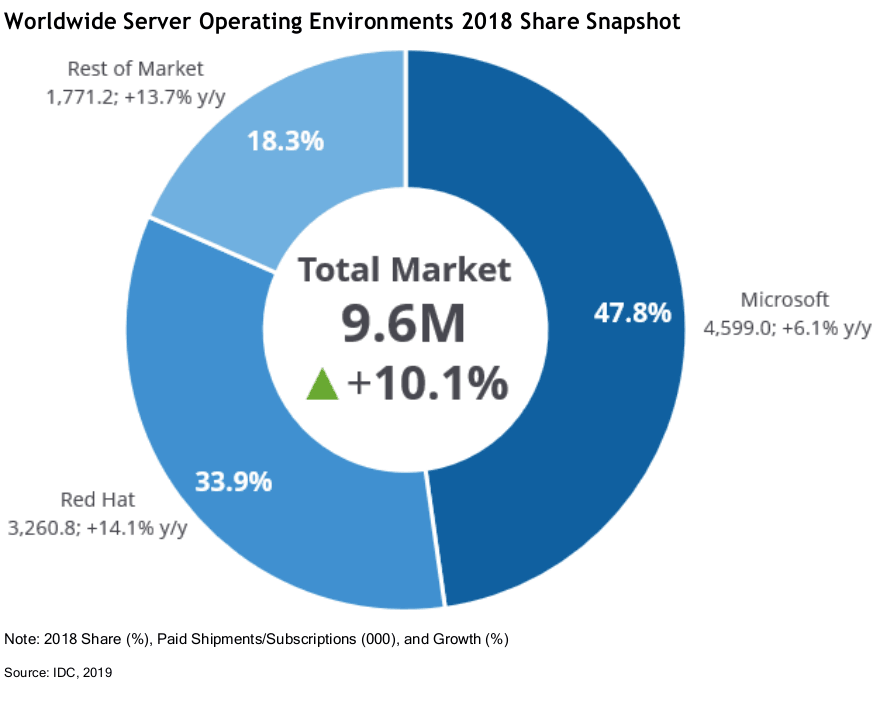
\includegraphics[width=0.8\textwidth]{figures/server-operating-system-market-share-2018.png}
    \caption{Operating Systems for Servers Market Share}
    \label{fig:Operating_Systems_for_Servers_Market_Share}
\end{figure}

As of 2018, Microsoft held 47.8\% of the market, while Red Hat held 33.9\%. 
The remaining 18.3\% of the market is shared by different competitors.   

\cite{ServerOsMarketShare}

\subsubsection{Market Volume}

Due to the rapid growth of the internet and related services, the market for servers and Operating Systems grew alongside it. 
It's expected to grow to double its current volume by 2032. 

\begin{figure}[H]
    \centering
    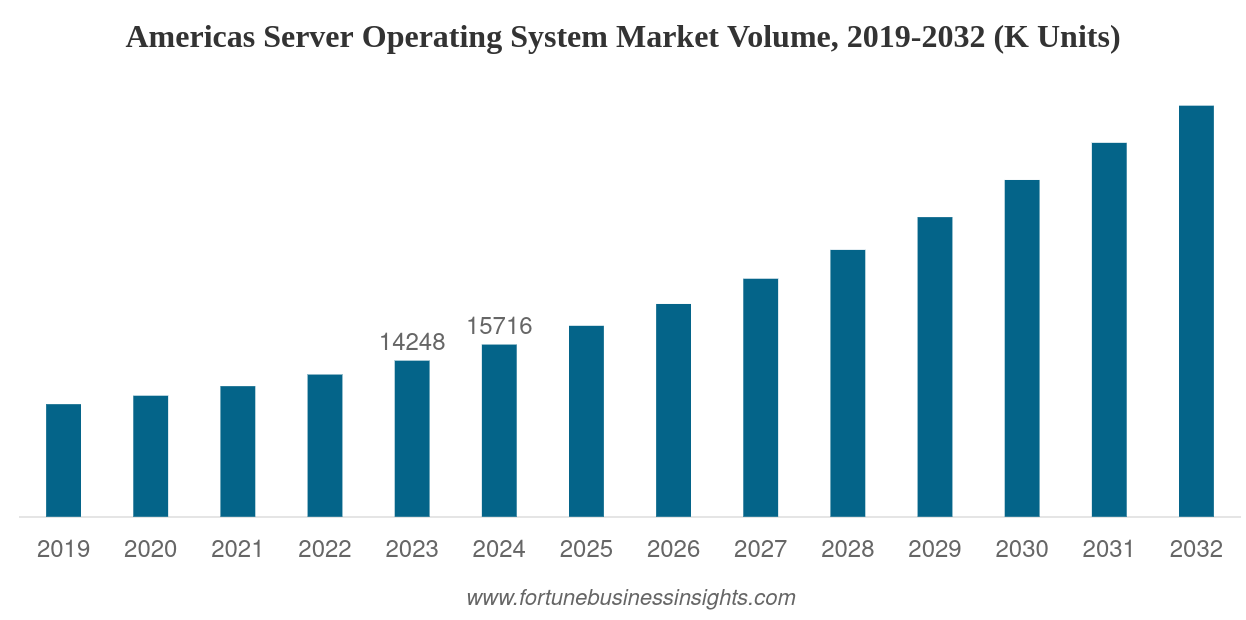
\includegraphics[width=0.8\textwidth]{figures/Server-Market-Volume.png}
    \caption{Operating Systems Market Volume}
    \label{fig:Operating_Systems_for_Servers_Market_Share}
\end{figure}

\cite{ServerOsMarketShare2}

\subsection{Operating Systems for Embedded Systems}

Embedded Systems are also a big market for Operating Systems. These are compact systems that are used in many different devices.
The CAGR for the Embedded Systems Market is expected to be 6.65\% from 2023 to 2030. Thus, the market volume is expected to grow to \textdollar 9,519.09 million by 2028.
One of the largest markets for Embedded Systems is the automotive industry. 

\cite{EmbeddedOsMarketShare}

\section{Important Players}

There are many different companies that develop Operating Systems. In this section, some of the most important ones will be discussed.

\subsection{Microsoft}

Microsoft is one of the biggest players in the OS market. They are most widely known for their Windows OS.
The company was founded by Bill Gates and Paul Allen in 1975. The company is headquartered in Redmond, Washington.

The company has a market capitalization of 2.5 trillion dollars. 

They currently hold 47.8\% of the Server OS Market and 70.62\% of the Desktop OS Market.
They are also active in the Server OS Market with Windows Server and the Embedded Systems Market with their Windows Embedded OS. 

\cite{Microsoft}
\cite{DesktopOsMarketShare}

\subsection{Apple}

Apple is another big player in the OS market. They are known for their macOS for desktop computers and iOS for their phones and tablets.
The company was founded by Steve Jobs, Steve Wozniak, and Ronald Wayne in 1976. The company is headquartered in Cupertino, California.

The company has a market capitalization of 2.5 trillion dollars. They currently hold 15.74\% of the Desktop OS Market and 27.78\% of the Mobile OS Market.

\cite{AppleOnWikipedia}

\subsection{Red Hat}

Red Hat specializes in Linux-based Operating Systems. The company was founded in 1993 and is headquartered in Raleigh, North Carolina.
The company was acquired by IBM in 2019 for 34 billion dollars.

They are the second biggest player in the Server OS Market with a market share of 33.9\%. 
Due to its open-source nature, Red Hat has a large community of developers contributing to the OS growth.

\cite{RedHatWiki}

\subsection{Wind River Systems}

Wind River Systems is a company that specializes in Embedded Systems. The company is known for its VxWorks OS. The system is used in many different industries like automotive, aerospace, defense, and industrial.
The company was founded in 1981 and is headquartered in Alameda, California.

They used to be a subsidiary of TPG Capital but were sold to Aptiv in 2022 for \textdollar 3.5 billion dollars.

\cite{WindriverSold}
\cite{Windriver}


\section{Conclusion}

The Market for Operating Systems in all relevante branches of the Industrie has been steadily growing over the last decade.
Due to the high amount of competition there has been constant development of the technology. 
This trend is expected to persist as digitalization becomes more integrated into everyday life and industries continue to demand more sophisticated and specialized Operating Systems. With emerging technologies like cloud computing, artificial intelligence, and the Internet of Things (IoT), new opportunities for OS development and market expansion are constantly arising.

Moreover, the competition between major OS developers ensures continuous innovation and improvement in performance, security, and user experience. Companies are investing heavily in research and development to maintain their market positions and adapt to evolving consumer and enterprise needs.

In conclusion, the Operating System market remains a vital and dynamic sector in the global economy. Its influence extends beyond traditional computing devices, shaping the future of technological progress across various industries.

\author{Florian Prandstetter}
